\documentclass{standalone}
\usepackage{tikz}
\usetikzlibrary{patterns, positioning}
\usetikzlibrary{shapes.misc}
\usepackage[outline]{contour}
\contourlength{1.5pt} 


\begin{document}
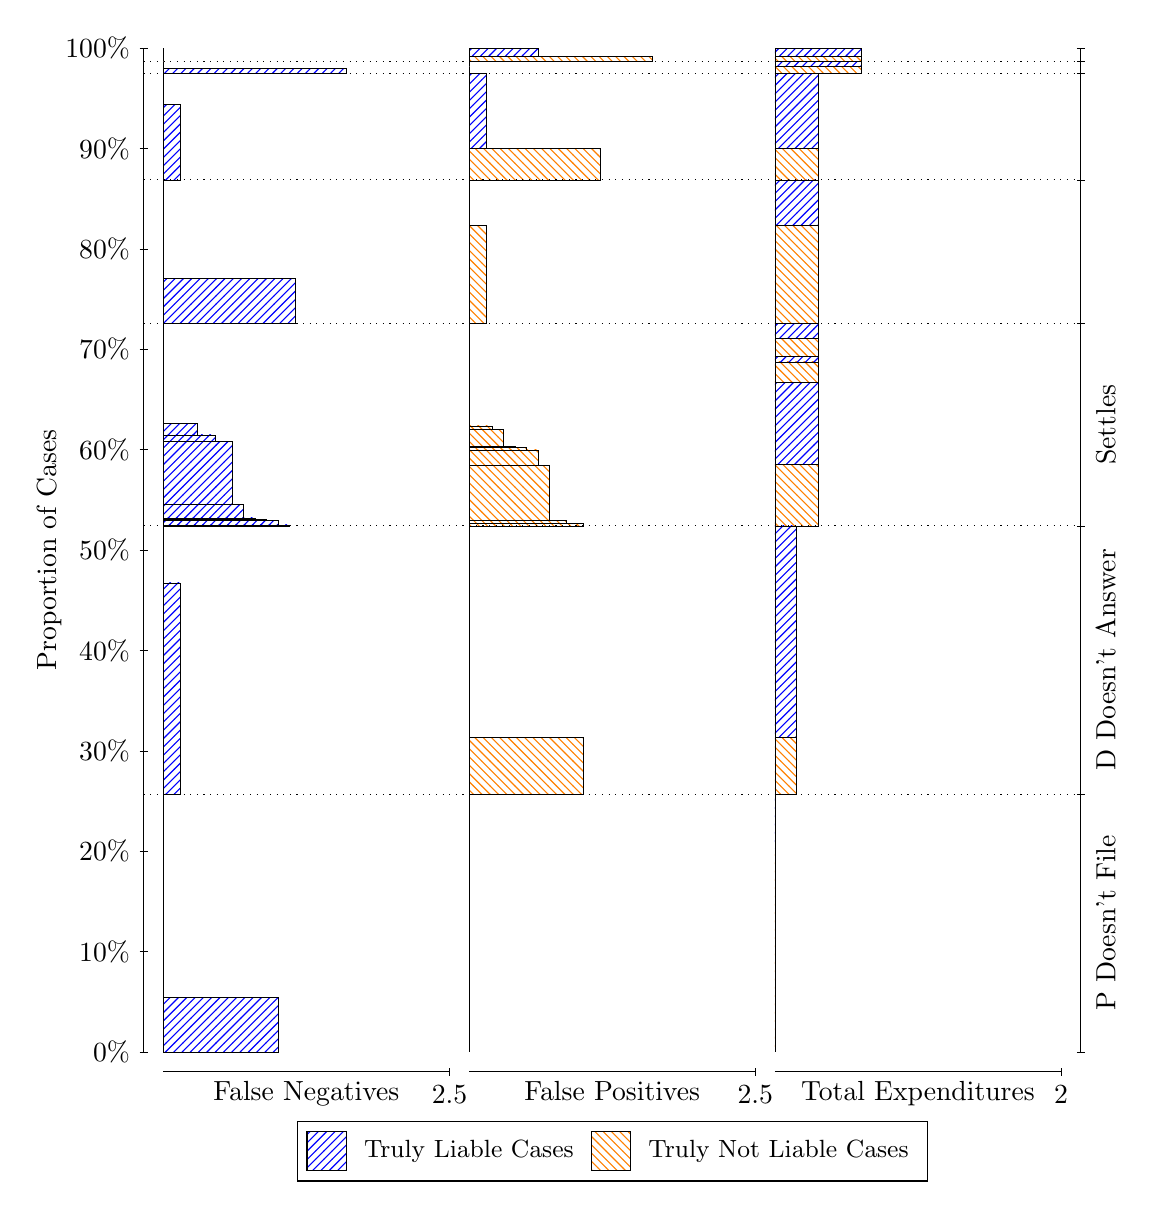
\begin{tikzpicture}
\draw[black, very thin] (1.5,1.75) -- (1.5,14.5);
\node[rotate=90, text=black, anchor=center] at (0.3, 8.125) {Proportion of Cases};
\draw[black, very thin] (1.45,1.75) -- (1.55,1.75);
\node[text=black, anchor=east] at (1.45, 1.75) {0\%};
\draw[black, very thin] (1.45,3.025) -- (1.55,3.025);
\node[text=black, anchor=east] at (1.45, 3.025) {10\%};
\draw[black, very thin] (1.45,4.3) -- (1.55,4.3);
\node[text=black, anchor=east] at (1.45, 4.3) {20\%};
\draw[black, very thin] (1.45,5.575) -- (1.55,5.575);
\node[text=black, anchor=east] at (1.45, 5.575) {30\%};
\draw[black, very thin] (1.45,6.85) -- (1.55,6.85);
\node[text=black, anchor=east] at (1.45, 6.85) {40\%};
\draw[black, very thin] (1.45,8.125) -- (1.55,8.125);
\node[text=black, anchor=east] at (1.45, 8.125) {50\%};
\draw[black, very thin] (1.45,9.4) -- (1.55,9.4);
\node[text=black, anchor=east] at (1.45, 9.4) {60\%};
\draw[black, very thin] (1.45,10.675) -- (1.55,10.675);
\node[text=black, anchor=east] at (1.45, 10.675) {70\%};
\draw[black, very thin] (1.45,11.95) -- (1.55,11.95);
\node[text=black, anchor=east] at (1.45, 11.95) {80\%};
\draw[black, very thin] (1.45,13.225) -- (1.55,13.225);
\node[text=black, anchor=east] at (1.45, 13.225) {90\%};
\draw[black, very thin] (1.45,14.5) -- (1.55,14.5);
\node[text=black, anchor=east] at (1.45, 14.5) {100\%};

\draw[black, very thin] (13.4,1.75) -- (13.4,14.5);
\draw[black, very thin] (13.35,1.75) -- (13.45,1.75);
\node[anchor=west] at (13.35, 1.75) {};
\draw[black, very thin] (13.35,5.0243) -- (13.45,5.0243);
\node[anchor=west] at (13.35, 5.0243) {};
\draw[black, very thin] (13.35,8.4313) -- (13.45,8.4313);
\node[anchor=west] at (13.35, 8.4313) {};
\draw[black, very thin] (13.35,11) -- (13.45,11);
\node[anchor=west] at (13.35, 11) {};
\draw[black, very thin] (13.35,12.825) -- (13.45,12.825);
\node[anchor=west] at (13.35, 12.825) {};
\draw[black, very thin] (13.35,14.178) -- (13.45,14.178);
\node[anchor=west] at (13.35, 14.178) {};
\draw[black, very thin] (13.35,14.329) -- (13.45,14.329);
\node[anchor=west] at (13.35, 14.329) {};
\draw[black, very thin] (13.35,14.5) -- (13.45,14.5);
\node[anchor=west] at (13.35, 14.5) {};

\draw[black, very thin, pattern color=blue, pattern=north east lines] (1.75,1.75) rectangle (3.2033,2.4455);
\draw[black, very thin, pattern color=orange, pattern=north west lines] (1.75,2.4455) rectangle (1.75,5.0243);
\draw[black, very thin, pattern color=blue, pattern=north east lines] (1.75,5.0243) rectangle (1.968,7.7064);
\draw[black, very thin, pattern color=orange, pattern=north west lines] (1.75,7.7064) rectangle (1.75,8.4313);
\draw[black, very thin, pattern color=blue, pattern=north east lines] (1.75,8.4313) rectangle (3.3487,8.4429);
\draw[black, very thin, pattern color=blue, pattern=north east lines] (1.75,8.4429) rectangle (3.2033,8.5021);
\draw[black, very thin, pattern color=blue, pattern=north east lines] (1.75,8.5021) rectangle (3.058,8.5113);
\draw[black, very thin, pattern color=blue, pattern=north east lines] (1.75,8.5113) rectangle (2.9127,8.5321);
\draw[black, very thin, pattern color=blue, pattern=north east lines] (1.75,8.5321) rectangle (2.7673,8.6995);
\draw[black, very thin, pattern color=blue, pattern=north east lines] (1.75,8.6995) rectangle (2.622,9.502);
\draw[black, very thin, pattern color=blue, pattern=north east lines] (1.75,9.502) rectangle (2.404,9.5876);
\draw[black, very thin, pattern color=blue, pattern=north east lines] (1.75,9.5876) rectangle (2.186,9.7284);
\draw[black, very thin, pattern color=orange, pattern=north west lines] (1.75,9.7284) rectangle (1.75,11);
\draw[black, very thin, pattern color=blue, pattern=north east lines] (1.75,11) rectangle (3.4213,11.575);
\draw[black, very thin, pattern color=orange, pattern=north west lines] (1.75,11.575) rectangle (1.75,12.825);
\draw[black, very thin, pattern color=blue, pattern=north east lines] (1.75,12.825) rectangle (1.968,13.782);
\draw[black, very thin, pattern color=orange, pattern=north west lines] (1.75,13.782) rectangle (1.75,14.178);
\draw[black, very thin, pattern color=blue, pattern=north east lines] (1.75,14.178) rectangle (4.0753,14.242);
\draw[black, very thin, pattern color=orange, pattern=north west lines] (1.75,14.242) rectangle (1.75,14.329);
\draw[black, very thin, pattern color=orange, pattern=north west lines] (1.75,14.329) rectangle (1.75,14.397);
\draw[black, very thin, pattern color=blue, pattern=north east lines] (1.75,14.397) rectangle (1.75,14.5);
\draw[black, very thin, pattern color=orange, pattern=north west lines] (5.6333,1.75) rectangle (5.6333,4.3288);
\draw[black, very thin, pattern color=blue, pattern=north east lines] (5.6333,4.3288) rectangle (5.6333,5.0243);
\draw[black, very thin, pattern color=orange, pattern=north west lines] (5.6333,5.0243) rectangle (7.0867,5.7492);
\draw[black, very thin, pattern color=blue, pattern=north east lines] (5.6333,5.7492) rectangle (5.6333,8.4313);
\draw[black, very thin, pattern color=orange, pattern=north west lines] (5.6333,8.4313) rectangle (7.0867,8.4601);
\draw[black, very thin, pattern color=orange, pattern=north west lines] (5.6333,8.4601) rectangle (6.8687,8.5008);
\draw[black, very thin, pattern color=orange, pattern=north west lines] (5.6333,8.5008) rectangle (6.6507,9.1969);
\draw[black, very thin, pattern color=orange, pattern=north west lines] (5.6333,9.1969) rectangle (6.5053,9.3954);
\draw[black, very thin, pattern color=orange, pattern=north west lines] (5.6333,9.3954) rectangle (6.36,9.4236);
\draw[black, very thin, pattern color=orange, pattern=north west lines] (5.6333,9.4236) rectangle (6.2147,9.442);
\draw[black, very thin, pattern color=orange, pattern=north west lines] (5.6333,9.442) rectangle (6.0693,9.6559);
\draw[black, very thin, pattern color=orange, pattern=north west lines] (5.6333,9.6559) rectangle (5.924,9.7024);
\draw[black, very thin, pattern color=blue, pattern=north east lines] (5.6333,9.7024) rectangle (5.6333,11);
\draw[black, very thin, pattern color=orange, pattern=north west lines] (5.6333,11) rectangle (5.8513,12.249);
\draw[black, very thin, pattern color=blue, pattern=north east lines] (5.6333,12.249) rectangle (5.6333,12.825);
\draw[black, very thin, pattern color=orange, pattern=north west lines] (5.6333,12.825) rectangle (7.3047,13.221);
\draw[black, very thin, pattern color=blue, pattern=north east lines] (5.6333,13.221) rectangle (5.8513,14.178);
\draw[black, very thin, pattern color=orange, pattern=north west lines] (5.6333,14.178) rectangle (5.6333,14.265);
\draw[black, very thin, pattern color=blue, pattern=north east lines] (5.6333,14.265) rectangle (5.6333,14.329);
\draw[black, very thin, pattern color=orange, pattern=north west lines] (5.6333,14.329) rectangle (7.9587,14.397);
\draw[black, very thin, pattern color=blue, pattern=north east lines] (5.6333,14.397) rectangle (6.5053,14.5);
\draw[black, very thin, pattern color=orange, pattern=north west lines] (9.5167,1.75) rectangle (9.5167,4.3288);
\draw[black, very thin, pattern color=blue, pattern=north east lines] (9.5167,4.3288) rectangle (9.5167,5.0243);
\draw[black, very thin, pattern color=orange, pattern=north west lines] (9.5167,5.0243) rectangle (9.7892,5.7492);
\draw[black, very thin, pattern color=blue, pattern=north east lines] (9.5167,5.7492) rectangle (9.7892,8.4313);
\draw[black, very thin, pattern color=orange, pattern=north west lines] (9.5167,8.4313) rectangle (10.062,9.2153);
\draw[black, very thin, pattern color=blue, pattern=north east lines] (9.5167,9.2153) rectangle (10.062,10.253);
\draw[black, very thin, pattern color=orange, pattern=north west lines] (9.5167,10.253) rectangle (10.062,10.514);
\draw[black, very thin, pattern color=blue, pattern=north east lines] (9.5167,10.514) rectangle (10.062,10.585);
\draw[black, very thin, pattern color=orange, pattern=north west lines] (9.5167,10.585) rectangle (10.062,10.811);
\draw[black, very thin, pattern color=blue, pattern=north east lines] (9.5167,10.811) rectangle (10.062,11);
\draw[black, very thin, pattern color=orange, pattern=north west lines] (9.5167,11) rectangle (10.062,12.249);
\draw[black, very thin, pattern color=blue, pattern=north east lines] (9.5167,12.249) rectangle (10.062,12.825);
\draw[black, very thin, pattern color=orange, pattern=north west lines] (9.5167,12.825) rectangle (10.062,13.221);
\draw[black, very thin, pattern color=blue, pattern=north east lines] (9.5167,13.221) rectangle (10.062,14.178);
\draw[black, very thin, pattern color=orange, pattern=north west lines] (9.5167,14.178) rectangle (10.607,14.265);
\draw[black, very thin, pattern color=blue, pattern=north east lines] (9.5167,14.265) rectangle (10.607,14.329);
\draw[black, very thin, pattern color=orange, pattern=north west lines] (9.5167,14.329) rectangle (10.607,14.397);
\draw[black, very thin, pattern color=blue, pattern=north east lines] (9.5167,14.397) rectangle (10.607,14.5);
\draw[black, dotted] (1.5,5.0243) -- (13.4,5.0243);
\draw[black, dotted] (1.5,8.4313) -- (13.4,8.4313);
\draw[black, dotted] (1.5,11) -- (13.4,11);
\draw[black, dotted] (1.5,12.825) -- (13.4,12.825);
\draw[black, dotted] (1.5,14.178) -- (13.4,14.178);
\draw[black, dotted] (1.5,14.329) -- (13.4,14.329);
\draw[black, very thin] (1.75,1.5) -- (5.3833,1.5);
\node[text=black, anchor=north] at (3.5667, 1.5) {False Negatives};
\draw[black, very thin] (5.3833,1.45) -- (5.3833,1.55);
\node[text=black, anchor=north] at (5.3833, 1.45) {2.5};

\draw[black, very thin] (5.6333,1.5) -- (9.2667,1.5);
\node[text=black, anchor=north] at (7.45, 1.5) {False Positives};
\draw[black, very thin] (9.2667,1.45) -- (9.2667,1.55);
\node[text=black, anchor=north] at (9.2667, 1.45) {2.5};

\draw[black, very thin] (9.5167,1.5) -- (13.15,1.5);
\node[text=black, anchor=north] at (11.333, 1.5) {Total Expenditures};
\draw[black, very thin] (13.15,1.45) -- (13.15,1.55);
\node[text=black, anchor=north] at (13.15, 1.45) {2};

\node[text=black, centered, rotate=90] at (13.72, 3.3871) {\contour{white}{P Doesn't File}};
\node[text=black, centered, rotate=90] at (13.72, 6.7278) {\contour{white}{D Doesn't Answer}};
\node[text=black, centered, rotate=90] at (13.72, 9.7154) {\contour{white}{Settles}};





\draw (7.449999999999999,1.5) node[draw=none] (baseCoordinate) {};
\begin{scope}[align=center]
        \matrix[scale=0.5, draw=black, below=0.5cm of baseCoordinate, nodes={draw}, column sep=0.1cm]{
            \node[rectangle, draw, minimum width=0.5cm, minimum height=0.5cm, pattern color=blue, pattern=north east lines] {}; &
            \node[draw=none, font=\small, text=black] (B) {Truly Liable Cases}; &
            \node[rectangle, draw, minimum width=0.5cm, minimum height=0.5cm, pattern color=orange, pattern=north west lines] {}; &
            \node[draw=none, font=\small, text=black] (B) {Truly Not Liable Cases}; \\
            };
\end{scope}

\end{tikzpicture}
\end{document}